\documentclass{article}

\usepackage{amsmath}
\usepackage{tikz}
\usepackage{mathtools}
\usepackage{amsfonts}
\usepackage{program}
\usepackage{cite}
\usepackage{csvsimple}
\usepackage{booktabs}
\usepackage[justification=centering]{caption}
\renewcommand{\arraystretch}{2}

\newcommand\todo[1]{\textcolor{red}{#1}}
\newcommand\opt{\textsc{opt}}
\newcommand\us{\textsc{us}}
\newcommand\E[1]{E \lbrack #1 \rbrack}
\newcommand\mspan[1]{\textbf{span}(#1)}
\newcommand{\proj}[2][]{\textbf{proj}_{#1}#2}
\newcommand\norm[1]{\|#1\|}

\DeclarePairedDelimiter{\ceil}{\lceil}{\rceil}
\DeclarePairedDelimiter{\floor}{\lfloor}{\rfloor}

\usepackage{listings}
\usepackage[T1]{fontenc}
\newcommand\BeraMonottfamily{%
  \def\fvm@Scale{0.6}% scales the font down
  \fontfamily{fvm}\selectfont% selects the Bera Mono font
}

\definecolor{keywords}{RGB}{255,0,90}
\definecolor{comments}{RGB}{0,0,113}
\definecolor{red}{RGB}{160,0,0}
\definecolor{green}{RGB}{0,150,0}

\definecolor{codegreen}{rgb}{0,0.6,0}
\definecolor{codegray}{rgb}{0.5,0.5,0.5}
\definecolor{codepurple}{rgb}{0.58,0,0.82}
\definecolor{backcolour}{rgb}{0.95,0.95,0.92}

\lstdefinestyle{mystyle}{
  commentstyle=\color{codegreen},
  keywordstyle=\color{magenta},
  numberstyle=\tiny\color{codegray},
  stringstyle=\color{codepurple},
  basicstyle=\BeraMonottfamily\footnotesize,
  breakatwhitespace=false,
  breaklines=true,
  captionpos=b,
  keepspaces=true,
  numbers=left,
  numbersep=8pt,
  showspaces=false,
  showstringspaces=false,
  showtabs=false,
  tabsize=2
}

\lstset{language=Python,
  style=mystyle}

\renewcommand{\thesection}{Question \arabic{section}.}
\renewcommand{\thesubsection}{\alph{subsection}}
\renewcommand{\thesubsubsection}{\arabic{subsubsection}}

\allowdisplaybreaks

\begin{document}

\title{CS690OP midterm}
\maketitle

\section{Rosenbrock's Function}

\subsection{Steepest Descent}

Figure \ref{fig:rosenbrock-linear} shows the convergence of the method of steepest descent for a variety of different starting points and step sizes. Steepest descent doesn't usually converge unless the step size is very small ($< 0.0014$ in my rough tests), and takes a few thousand iterations to do so.

\begin{figure}[!ht]
  \centering
  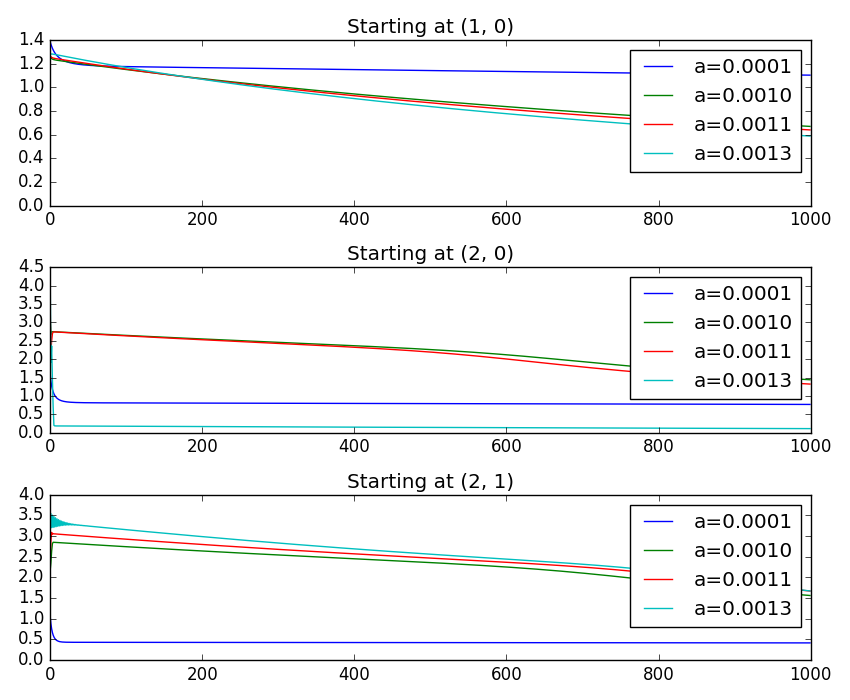
\includegraphics[width=\textwidth,keepaspectratio=true]{rosenbrock-linear.png}
  \caption{Convergence of Steepest Descent, for various starting points and step sizes}
  \label{fig:rosenbrock-linear}
\end{figure}

\subsection{Newton's Method}

Figure \ref{fig:rosenbrock-newtons} shows the convergence rate of Newton's Method. This method converges almost instantly (within 6 or 7 steps), no matter where we start from.

\begin{figure}[!ht]
  \centering
  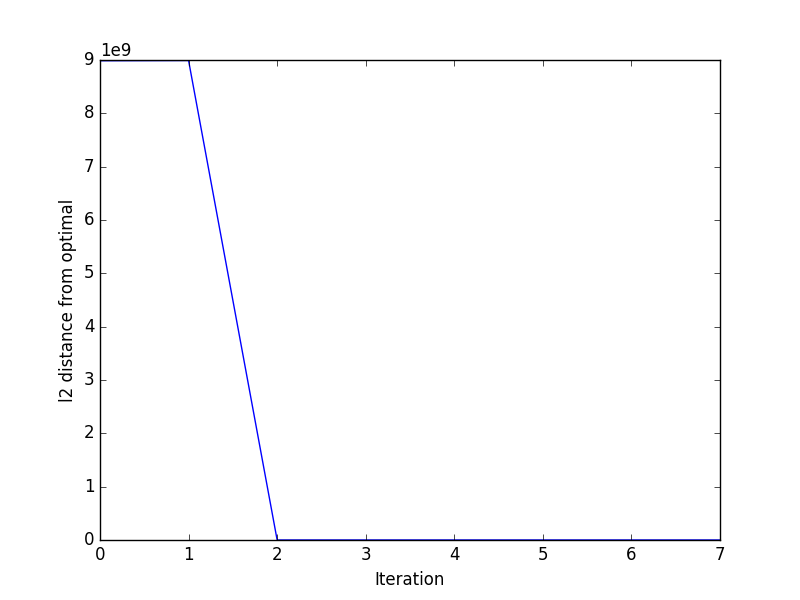
\includegraphics[width=\textwidth,keepaspectratio=true]{rosenbrock-newtons.png}
  \caption{Convergence of Newton's Method on the Rosenbrock Function, starting from $(-52970, -2159)$}
  \label{fig:rosenbrock-newtons}
\end{figure}

\section{Subgradients}

\subsection{Subgradient of Max}

\todo{this}

\subsection{Projected Subgradient}

To project onto the line segment, we can first project onto the line $x_1 + x_2 = 1$. If $x_1,x_2 > 0$, then we have the projection onto the line segment. If $x_1 < 0$, we can use the point $(0, 1)$. Otherwise, we can use the point $(1, 0)$.

Here's a proof that this method of projection works for the $L-2$ norm. Since we are just trying to keep the gradient descent in the feasible region, we can use any norm that is convenient.

Let $\proj[L]{x}$ be the projection of a point $x$ onto the line $x_1 + x_2 = 1$. Suppose our method projected the point onto $p_1$ which has a distance $d_1$, but the actual nearest was $p_2$ with a distance $d_2 < d_1$. Let $\Delta_1 = \norm{p_1 - \proj[L]{x}}_2$, let $\Delta_2 = \norm{p_2 - \proj[L]{x}}_2$, and let $h = \norm{x - \proj[L]{x}}_2$. Since we pick the nearest point to $\proj[L]{x}$ on the line segment, $\epsilon = \Delta_2 - \Delta_1 \geq 0$. By the pythagorean theorem, $d_1^2 = \Delta_1^2 + h^2$ and $d_2^2 = \Delta_1^2 + h^2 = (\Delta_1 + \epsilon)^2 + h^2 = \Delta_1^2 + 2\Delta_1 \epsilon + \epsilon^2 + h^2 \geq d_1$, which is a contradiction.

Starting from $(0,1)$, the gradient step takes us to $(-1, -1)$, which is projected to $(0.5, 0.5)$. The next gradient step takes us to $(-1.5, 1)$, which is projected to $(1,0)$ which is optimal.

\begin{figure}[!ht]
  \centering
  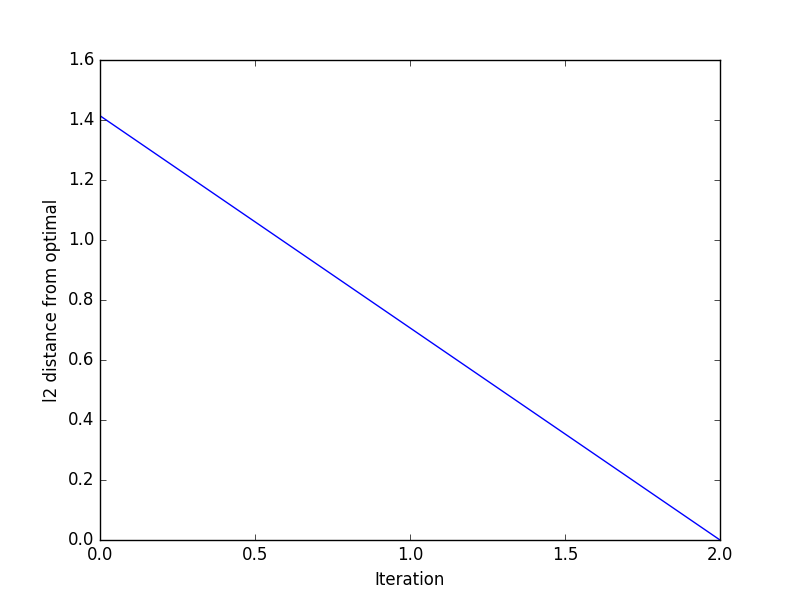
\includegraphics[width=\textwidth,keepaspectratio=true]{projected-descent.png}
  \caption{Convergence of Projected Gradient Descent}
  \label{fig:projected-descent}
\end{figure}

\section{Kaczmarz}

Figure \ref{fig:kaczmarz} shows the convergence of the different kaczmarz methods for $A = \begin{bmatrix}1 & 0 & 1 \\ 0 & 1 & 1 \\ 1 & 1 & 0\end{bmatrix}$ and $b$ picked as a random number in the range $\lbrack 0, 1)$.

  \begin{figure}[!ht]
    \centering
    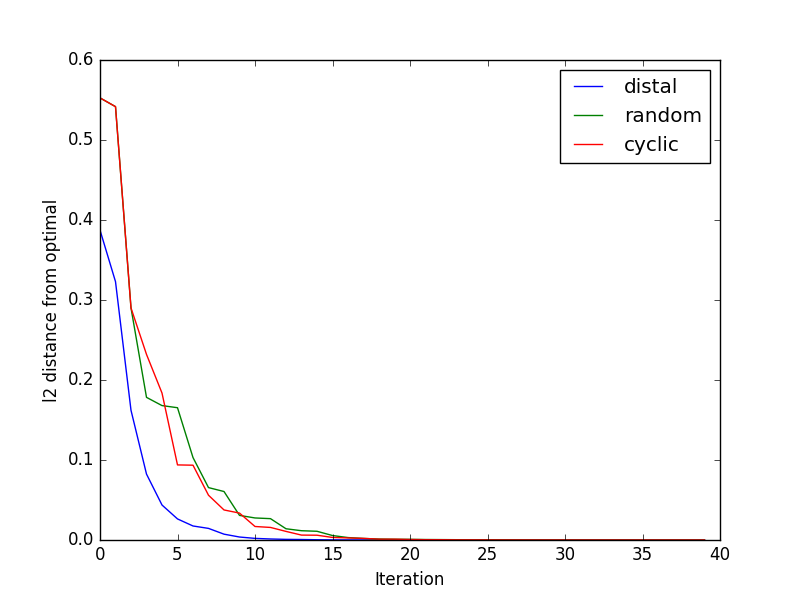
\includegraphics[width=\textwidth,keepaspectratio=true]{kaczmarz.png}
    \caption{Convergence of different kaczmarz methods for a 3x3 $A$ and a random starting $b$}
    \label{fig:kaczmarz}
\end{figure}

For the same $A$ and $b = \begin{bmatrix}0.3467 & 0.8979 & 0.9461\end{bmatrix}^T$, the distal method outperforms all the others. The distal method converges in 14 iterations, while the random method converges in 28, and the cyclic method takes > 2000.

\section{Oblique Projections}

\subsection{Example 1}

$w_{\text{best}} = \frac{1}{5}r_1 + \frac{2+\gamma}{5(1-\gamma)}r_2$
$w_{\text{TD}} = \frac{r_1+2r_2}{5-6\gamma}$
$w_{\text{BR}} = \frac{(1-2\gamma)r_1+(2-2\gamma)r_2}{(1-2\gamma)^2+(2-2\gamma)^2}$

I did the omitted algebraic steps to find $\frac{e(w_X)}{e(w_{\text{best}})}$ for both $TD$ and $BR$.

For $TD$, $\frac{e(w_{\text{TD}})}{e(w_{\text{best}})} = \frac{5(5-12\gamma + 9\gamma^2)}{(5 - 6 \gamma)^2}$. This confirms that the $TD$ error ratio is independent of $r_1$ and $r_2$. As $\gamma$ approaches $\frac{5}{6}$, the denominator of the $TD$ error ratio approaches 0, and the error ratio approaches infinity.

For $BR$, $\frac{e(w_{\text{BR}})}{e(w_{\text{best}})} = \frac{5 \left(16 g^4-40 g^3+45 g^2-24 g+5\right)}{\left(8 g^2-12 g+5\right)^2}$. This confirms that the $BR$ error ratio is also independent of $r_1$ and $r_2$. As $\gamma$ approaches $\frac{5}{6}$, the denominator of this error ratio approaches $\frac{25}{81}$, so the error ratio is bounded. In fact, over the interval $\gamma = (0,1)$, the error ratio is always below 14.

\subsection{How the methods use oblique projections}

Both methods estimate the value of $v$ with a linear combination of features $\phi$. They do this by obliquely projecting $v$ onto $\mspan{\Phi}$. The resulting vector $\hat{v}$ is a linear combination of the different features which is nearest to $v$ in some sense. Instead of doing the orthogonal projection onto $\mspan{\Phi}$, both $TD$ and $BR$ find the vector on $\mspan{\Phi}$ which is orthogonal to some other surface $\mspan{L^TX}$.

The value of $X$ is different for each method. Let $\Xi$ be a diagonal matrix of a probability distribution over the states of the system, $r$ be a vector of rewards, and $L$ be a matrix where $v = L^{-1}r$. $TD$ finds the vector orthogonal to $\mspan{L^T\Xi\Phi}$, while $BR$ finds the vector orthogonal to $\mspan{L^T\Xi L \Phi}$.

For example 1 in the paper, we have the following values for the variables:

\begin{align}
P &= \begin{bmatrix}
  0 & 1 \\
  0 & 1
\end{bmatrix} \\
L &= \begin{bmatrix}
  1 & 0 \\
  -\gamma & 1-\gamma
\end{bmatrix} \\
\Xi &= \begin{bmatrix}
  0.5 & 0 \\
  0 & 0.5
\end{bmatrix} \\
\Phi &= \begin{bmatrix}
  1 \\
  2
\end{bmatrix}
\end{align}

This means we have the following values for $X_{TD}$ and $X_{BR}$, which suggests that $X_{BR} = X_{TD} - \vec{\gamma}$

\begin{align}
  X_{TD} &= \Xi\Phi \\
  &= \begin{bmatrix}
    0.5 & 0 \\
    0 & 0.5
  \end{bmatrix} \begin{bmatrix}
    1 \\
    2
  \end{bmatrix} \\
  &= \begin{bmatrix}
    0.5 \\
    1
  \end{bmatrix} \\
  X_{BR} &= \Xi L \Phi \\
  &= \begin{bmatrix}
    0.5 & 0 \\
    0 & 0.5
  \end{bmatrix} \begin{bmatrix}
    1 & 0 \\
    -\gamma & 1-\gamma
  \end{bmatrix} \begin{bmatrix}
    1 \\
    2
  \end{bmatrix} \\
  &= \begin{bmatrix}
    0.5 - \gamma \\
    1 - \gamma
  \end{bmatrix}
\end{align}

\section{Matrix Completion}

See Table \ref{tab:rmse} for the RMSE for the different algorithms, Figure \ref{fig:convergence-factorization} for the convergence of the Factorization algorithm, and Figure \ref{fig:convergence-svt} for the convergence of the SVT algorithm.

I implemented the three baseline methods and the three more advanced methods in python using numpy. See \textsc{movielens/methods.py} for the implementation. A list of the parameters I used is in Table \ref{tab:params}.

For the factorization algorithm, I used a method from \cite{algorithmsNMF} (sec. 5) instead of the provided method, which appears to be an equivalent version of gradient descent. The paper's formulation allowed me to write one update step per iteration as a few matrix operations instead of trying to do one update per row per iteration. This made things much, much faster.

\begin{minipage}{\linewidth}
  \centering
  \captionof{table}{Parameter Values} \label{tab:params}
  \csvautotabular{movielens/parameters.csv}
\end{minipage}


\begin{minipage}{\linewidth}
\centering
\captionof{table}{RMSE for various Matrix Completion algorithms} \label{tab:rmse}
\csvautotabular{movielens/table.csv}
\end{minipage}

\footnotetext{These algorithms were only run on the 100k dataset because they were incredibly slow on the 1M dataset}

\begin{figure}[!ht]
  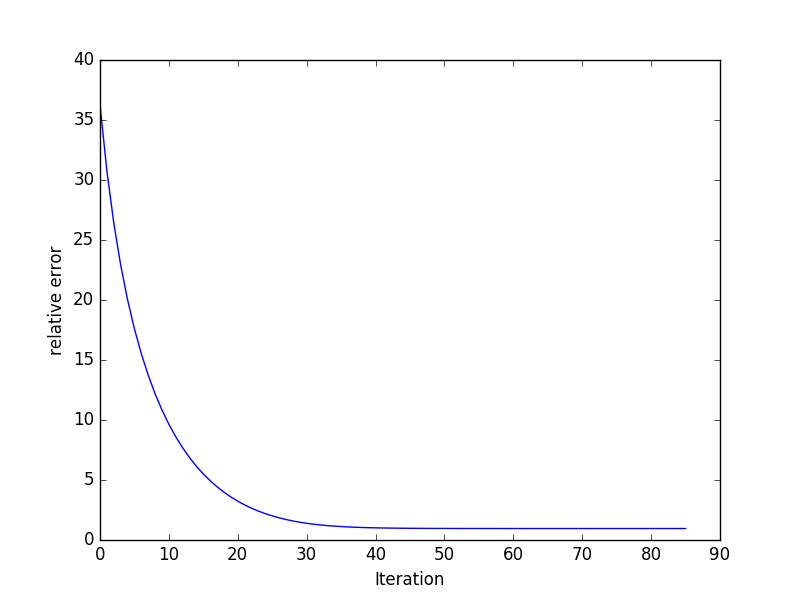
\includegraphics[width=\textwidth,keepaspectratio=true]{movielens/convergence-factorization-u2.png}
  \caption{Convergence of the factorization algorithm for 100k entries}
  \label{fig:convergence-factorization}
\end{figure}

\begin{figure}[!ht]
  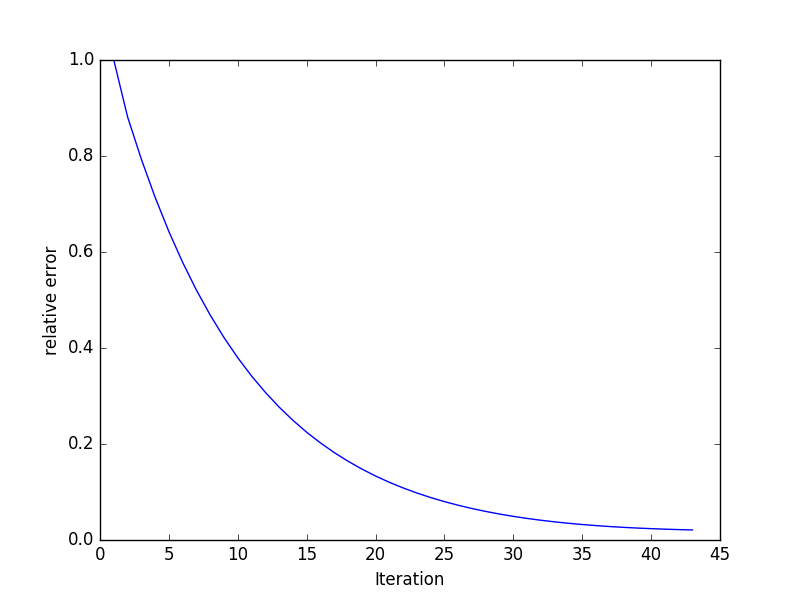
\includegraphics[width=\textwidth,keepaspectratio=true]{movielens/convergence-svt-u1.png}
  \caption{Convergence of the SVT algorithm for 100k entries}
  \label{fig:convergence-svt}
\end{figure}


\bibliography{writeup}{}
\bibliographystyle{plain}

\end{document}
